\documentclass{article}
\usepackage{amsmath}
\usepackage{amssymb}
\usepackage{graphicx}
\usepackage{hyperref}
\usepackage[version=4]{mhchem}

\title{Example 13}
\date{}

\begin{document}
\maketitle

\(A B\) is the diameter of semicircle \(O\). Extend \(A B\) to \(C\). \(D C\) is tangent to the semicircle at \(D . D E \perp A B . E\) is the foot of the perpendicular from \(D\) to \(A B . C D=2, A E=4 B E\). Find the length of \(B C\).\\
\centering
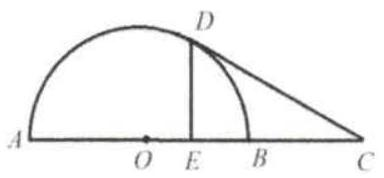
\includegraphics[width=\textwidth]{images/problem_image_1.jpg}

Solution: 1.\\
Connect \(O D\).\\
Let \(B E=x\).\\
\(O B=\frac{A B}{2}=\frac{A E+B E}{2}=\frac{5 B E}{2}=\frac{5 x}{2}\)\\
\centering
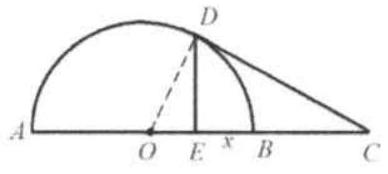
\includegraphics[width=\textwidth]{images/reasoning_image_1.jpg}\\
\(O E=O B-B E=\frac{A B}{2}-x=\frac{5 x}{2}-x=\frac{3 x}{2}\)\\
We know that\\
\(O D^{2}=O C \times O E\)\\
\(\Rightarrow\left(\frac{5 x}{2}\right)^{2}=\left(\frac{5 x}{2}+B C\right) \times \frac{3 x}{2}\)


\(\Rightarrow \frac{25 x}{6}=\frac{5 x}{2}+B C\)\\
\(\Rightarrow B C=\frac{25 x}{6}-\frac{5 x}{2}=\frac{25 x-15 x}{6}=\frac{5 x}{3}\)\\
We also know that\\
\(C D^{2}=A C \times B C\)\\
\(\Rightarrow 4=\left(5 x+\frac{5 x}{3}\right) \times \frac{5 x}{3}\)\\
\(\Rightarrow 4=\frac{9 x^{2}}{100} \quad \Rightarrow x^{2}=\frac{9}{25} \Rightarrow x=\frac{3}{5}\).\\
Thus \(B C=\frac{5 x}{3}=\frac{5}{3} \times \frac{3}{5}=1\).


\end{document}
